% Figure 1a of our false-alarm paper (rs2): the four target cues on DMD frames and a negative frame.
% All class boxes use solid lines.
\begin{tikzpicture}[font=\footnotesize]
\newcommand{\cuebox}[7]{% node, y0, x0, y1, x1, colour, label  (fractions of the image)
  \draw[#6, line width=1.4pt] ($(#1.south west)!#2!(#1.north west) + (#1.south west)!#3!(#1.south east) - (#1.south west)$) rectangle ($(#1.south west)!#4!(#1.north west) + (#1.south west)!#5!(#1.south east) - (#1.south west)$);
  \node[above right, fill=#6, text=white, inner sep=1.5pt, font=\scriptsize\bfseries] at ($(#1.south west)!#4!(#1.north west) + (#1.south west)!#3!(#1.south east) - (#1.south west)$) {#7};}
\node[inner sep=0pt] (i1) at (0,0) {
\includegraphics[width=3.0cm, height=3.0cm]{Figures/dmd/cue_yawn.jpg}};
\node[inner sep=0pt, right=0.35cm of i1] (i2) {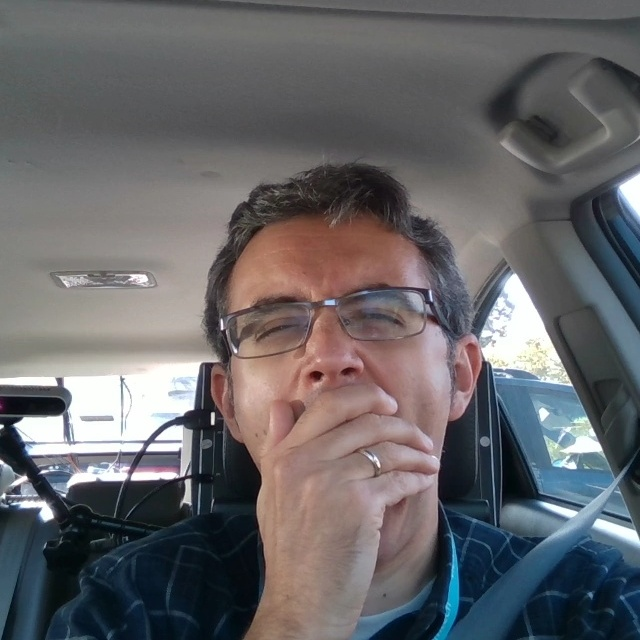
\includegraphics[width=3.0cm, height=3.0cm]{Figures/dmd/cue_hand_mouth.jpg}};
\node[inner sep=0pt, right=0.35cm of i2] (i3) {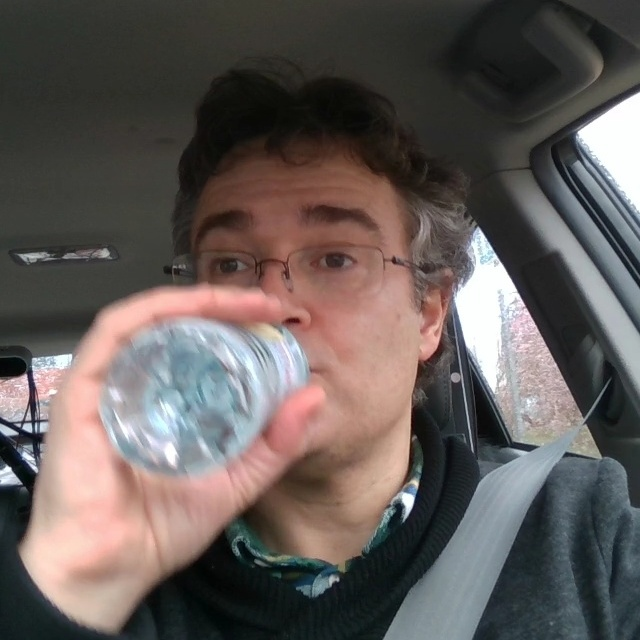
\includegraphics[width=3.0cm, height=3.0cm]{Figures/dmd/cue_drink.jpg}};
\node[inner sep=0pt, right=0.35cm of i3] (i4) {
\includegraphics[width=3.0cm, height=3.0cm]{Figures/dmd/cue_phone.jpg}};
\node[inner sep=0pt, right=0.35cm of i4] (i5) {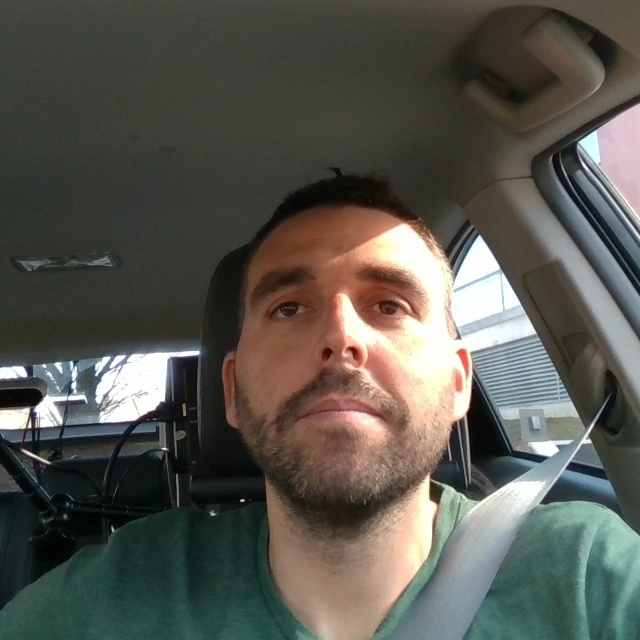
\includegraphics[width=3.0cm, height=3.0cm]{Figures/dmd/cue_negative.jpg}};
\cuebox{i1}{0.32}{0.46}{0.46}{0.67}{red!75!black}{yawn}
\cuebox{i2}{0.05}{0.38}{0.58}{0.70}{cyan!80!black}{hand-mouth}
\cuebox{i3}{0.22}{0.14}{0.56}{0.49}{teal!80!black}{drink}
\cuebox{i4}{0.22}{0.03}{0.63}{0.28}{violet!85!black}{phone}
\node[above left, fill=gray!80!black, text=white, inner sep=2pt, font=\scriptsize\bfseries] at ($(i5.north east) + (-0.08, -0.28)$) {No cue};
\node[below=3pt of i1, font=\small] {Yawning};
\node[below=3pt of i2, font=\small] {Hand-over-mouth};
\node[below=3pt of i3, font=\small] {Drinking};
\node[below=3pt of i4, font=\small] {Phone use};
\node[below=3pt of i5, font=\small] {Negative};
\end{tikzpicture}
